\documentclass[a4paper]{article}

% Compile from this directory (NLU/report/):
%   latexmk -pdf report_NLU.tex
% The style files are picked up from ../../report_template/.
\usepackage{../../report_template/INTERSPEECH2021}
\usepackage{booktabs}
\usepackage{pgfplots}
\pgfplotsset{compat=1.14}

% Colorblind-safe palette (Okabe-Ito).
\definecolor{cbblue}{HTML}{0072B2}
\definecolor{cbverm}{HTML}{D55E00}
\definecolor{cbgreen}{HTML}{009E73}
\definecolor{cbpurp}{HTML}{CC79A7}

% Self-contained bibliography: this block writes nlu_refs.bib at compile time.
\begin{filecontents*}[overwrite]{nlu_refs.bib}
@inproceedings{hemphill1990atis,
  author    = {Charles T. Hemphill and John J. Godfrey and George R. Doddington},
  title     = {The {ATIS} Spoken Language Systems Pilot Corpus},
  booktitle = {Speech and Natural Language: Proceedings of a Workshop Held at Hidden Valley},
  year      = {1990}
}
@inproceedings{ramshaw1995iob,
  author    = {Lance A. Ramshaw and Mitchell P. Marcus},
  title     = {Text Chunking Using Transformation-Based Learning},
  booktitle = {Third Workshop on Very Large Corpora},
  year      = {1995}
}
@article{radford2019gpt2,
  author  = {Alec Radford and Jeffrey Wu and Rewon Child and David Luan and Dario Amodei and Ilya Sutskever},
  title   = {Language Models are Unsupervised Multitask Learners},
  journal = {OpenAI Technical Report},
  year    = {2019}
}
@inproceedings{devlin2019bert,
  author    = {Jacob Devlin and Ming-Wei Chang and Kenton Lee and Kristina Toutanova},
  title     = {{BERT}: Pre-training of Deep Bidirectional Transformers for Language Understanding},
  booktitle = {Proceedings of NAACL-HLT},
  year      = {2019}
}
@article{chen2019bertjoint,
  author  = {Qian Chen and Zhu Zhuo and Wen Wang},
  title   = {{BERT} for Joint Intent Classification and Slot Filling},
  journal = {arXiv preprint arXiv:1902.10909},
  year    = {2019}
}
\end{filecontents*}

% Lab 5: Intent Classification and Slot Filling (parts 2.A and 2.B)
\title{NLU course project: Intent Classification and Slot Filling (Lab 5)}
\name{Kevin Shimaj (mat. 267432)}

\address{
  University of Trento}
\email{kevin.shimaj@studenti.unitn.it}

\begin{document}

\maketitle

\section{Introduction}
This report covers joint intent classification and slot filling on the ATIS corpus \cite{hemphill1990atis}, where a single model with two output heads predicts one intent per sentence and one IOB tag per word \cite{ramshaw1995iob}. In part 2.A the GPT-2 style decoder built for the language modeling project is adapted to the task: a word-level vocabulary replaces the BPE tokenizer, a classification token is appended at the end of each utterance, and the model is grown one hyperparameter at a time. The final configuration reaches a test slot F1 of $0.885 \pm 0.005$ and an intent accuracy of $0.929 \pm 0.004$ over five seeds. In part 2.B the pretrained BERT \cite{devlin2019bert} and GPT-2 \cite{radford2019gpt2} are fine-tuned on the same task, which moves the problem to the alignment between subword tokens and word-level slot labels; both clearly improve over part 2.A.

\section{Implementation details}
\textbf{Part 2.A.} All runs share the lab protocol: a 10\% development split stratified on the intent labels, a joint loss that sums the two cross entropies (a weighted sum $\lambda\,\mathcal{L}_{\text{slot}}+(1-\lambda)\mathcal{L}_{\text{intent}}$ is a possible variant, left at $\lambda{=}0.5$ here), slot loss that ignores padding, evaluation with the conll script for slots and accuracy for intents, and model selection on development slot F1. Since the model is a causal decoder, the classification token is appended at the end of the sentence, the only position that attends to every word; its slot label is set to the padding index so it never contributes to the slot loss. The search itself surfaced a protocol problem before any tuning could start: with 4.5k training sentences and batch size 128, one epoch is only 35 gradient updates, so a patience of 3 epochs, calibrated on PTB-sized epochs in the previous project, stopped every run after 4 to 6 epochs, inside an initial phase where the model predicts only the O tag and the entity-level F1 is stuck at zero. A diagnostic run with early stopping disabled (Figure~\ref{fig:diag}) showed a lucky peak at the first epoch, the zero-F1 phase, and then a smooth climb with improvement stalls of up to 10 epochs; the patience was therefore rescaled to 10, and epochs with zero F1 no longer consume it. Under this protocol the learning rate sweep on the tiny model selected $5\mathrm{e}{-3}$, with the grid extended to $1\mathrm{e}{-2}$ to close the optimum from above. During the capacity search, every step that regressed while showing instability inside the training curve (sudden drops of the development F1) received one extra run at $2\mathrm{e}{-3}$ before being reverted, since the learning rate chosen on the tiny model confounds the comparison: width 256 and a second layer recovered with the lower rate but stayed below the 128/1/1 model, while the feed-forward expansion to 512 was the only step where the check flipped the outcome. Dropout before the heads only hurt: no run ever showed the rise-then-decline signature of overfitting, so the extra regularization removed signal without curing anything.

\textbf{Part 2.B.} Both backbones keep the two heads and the data protocol of part 2.A, with the word vocabulary replaced by the pretrained tokenizers. One word maps to several subwords but has a single label, so labels are placed on the first subtoken of each word and every other position gets the ignore index of the loss, following \cite{chen2019bertjoint}; the mapping uses the tokenizer word alignment rather than manual splitting, and at evaluation time predictions are read only at first-subtoken positions and mapped back to the original words. The intent vector reflects each architecture: BERT reads the CLS token at position 0, since bidirectional attention sees the whole sentence from there, while GPT-2 reads the last real token, indexed through the attention mask with right padding. Both models are fully fine-tuned with AdamW. The BERT grid follows the values recommended by \cite{devlin2019bert}; repeated runs at a fixed seed measured a run-to-run variance of about 0.002 development F1, and all three rates fell inside it, so $5\mathrm{e}{-5}$ was chosen as the nominal best with the fastest convergence. The GPT-2 grid was also tied on development F1: $1\mathrm{e}{-4}$ was preferred because $5\mathrm{e}{-5}$ hit the epoch cap with the curve still rising and $2\mathrm{e}{-4}$ was noisier and weaker on test.

\section{Results}
Table~\ref{tab:parta} lists every part 2.A run, including the three killed by the miscalibrated early stopping, and Table~\ref{tab:partb} the part 2.B grid, where unintended fixed-seed replicas double as a measurement of run variance. The final scores over seeds 0 to 4 are in Table~\ref{tab:final}. Two observations. First, the part 2.A search rejected almost every capacity increase: on a small, closed-domain corpus the 128/1/1/512 decoder is already past the useful size, and the individual keep-or-revert margins are of the same order as the seed variance, so the final configuration should be read as equivalent to its neighbours rather than a clear winner. Model selection was on development slot F1 only, so the intent accuracy is not monotone across the log (it drops from 0.938 to 0.916 at the width step, Table~\ref{tab:parta}): the two heads share a backbone but are not co-selected, and the slot metric drives every decision. Second, the part 2.B gap over part 2.A ($+0.072$ slot F1 for BERT, $+0.036$ for GPT-2) is the transfer learning effect, and inside part 2.B BERT beats GPT-2 by $0.036$ slot F1 with a three times smaller seed variance: for sequence labeling each word benefits from its right context, which the bidirectional encoder sees and the causal decoder does not, while the gap on intent accuracy, where the whole sentence is available to both models, shrinks to $0.011$. Figure~\ref{fig:conv} compares the three convergence profiles.

{\footnotesize\noindent\textit{AI usage declaration}: a large language model was used to suggest the hyperparameter grids and to point to the {BERT} fine-tuning reference \cite{devlin2019bert}.\par}

% Keep the one-page body on page 1; send all tables, figures and references to page 2.
\clearpage

\begin{table}[t]
  \centering
  \caption{Part 2.A, full incremental log. Config is $d_{\mathrm{model}}$/heads/layers/ff. ES marks the early stopping protocol: v0 = lab patience 3, v1 = v0 plus zero-F1 guard, v2 = patience 10 plus guard (final), diag = early stopping disabled. Decision: K = kept, R = rejected.}
  \label{tab:parta}
  \scriptsize
  \setlength{\tabcolsep}{3.5pt}
  \begin{tabular}{@{}rllllllll@{}}
    \toprule
    \# & Step & ES & Config & lr & Dev F1 & Test F1 & Acc & D \\
    \midrule
    1  & lr sweep    & v0   & 20/1/1/20   & $1\mathrm{e}{-3}$ & 0.165 & 0.113 & 0.708 & R \\
    2  & lr sweep    & v0   & 20/1/1/20   & $5\mathrm{e}{-4}$ & 0.150 & 0.097 & 0.708 & R \\
    3  & lr sweep    & v1   & 20/1/1/20   & $1\mathrm{e}{-3}$ & 0.178 & 0.122 & 0.708 & R \\
    4  & diagnostic  & diag & 20/1/1/20   & $1\mathrm{e}{-3}$ & 0.917 & 0.863 & 0.916 & -- \\
    5  & lr sweep    & v2   & 20/1/1/20   & $1\mathrm{e}{-3}$ & 0.924 & 0.858 & 0.919 & K \\
    6  & lr sweep    & v2   & 20/1/1/20   & $5\mathrm{e}{-4}$ & 0.850 & 0.791 & 0.885 & R \\
    7  & lr sweep    & v2   & 20/1/1/20   & $5\mathrm{e}{-3}$ & 0.942 & 0.880 & 0.938 & K \\
    8  & lr sweep    & v2   & 20/1/1/20   & $1\mathrm{e}{-2}$ & 0.940 & 0.883 & 0.934 & R \\
    9  & $d_{\mathrm{model}}$ & v2 & 128/1/1/20 & $5\mathrm{e}{-3}$ & 0.945 & 0.895 & 0.916 & K \\
    10 & $d_{\mathrm{model}}$ & v2 & 256/1/1/20 & $5\mathrm{e}{-3}$ & 0.898 & 0.845 & 0.897 & R \\
    11 & lr check    & v2   & 256/1/1/20  & $2\mathrm{e}{-3}$ & 0.936 & 0.884 & 0.907 & R \\
    12 & heads       & v2   & 128/4/1/20  & $5\mathrm{e}{-3}$ & 0.939 & 0.893 & 0.909 & R \\
    13 & layers      & v2   & 128/1/2/20  & $5\mathrm{e}{-3}$ & 0.938 & 0.886 & 0.935 & R \\
    14 & lr check    & v2   & 128/1/2/20  & $2\mathrm{e}{-3}$ & 0.941 & 0.886 & 0.933 & R \\
    15 & ff ($4 \times d$) & v2 & 128/1/1/512 & $5\mathrm{e}{-3}$ & 0.941 & 0.889 & 0.925 & R \\
    16 & lr check    & v2   & 128/1/1/512 & $2\mathrm{e}{-3}$ & \textbf{0.949} & 0.889 & 0.928 & K \\
    17 & dropout 0.1 & v2   & 128/1/1/512 & $2\mathrm{e}{-3}$ & 0.938 & 0.885 & 0.937 & R \\
    \bottomrule
  \end{tabular}
\end{table}

\begin{table}[t]
  \centering
  \caption{Part 2.B, learning rate grids (seed 42). Rows marked rep.\ are unintended fixed-seed replicas; their spread measures the run-to-run variance. Decision: K = kept, R = rejected.}
  \label{tab:partb}
  \footnotesize
  \begin{tabular}{@{}rlllllll@{}}
    \toprule
    \# & Model & lr & Dev F1 & Test F1 & Acc & D \\
    \midrule
    1 & BERT & $2\mathrm{e}{-5}$        & 0.9805 & 0.9486 & 0.9731 & R \\
    2 & BERT & $2\mathrm{e}{-5}$ (rep.) & 0.9823 & 0.9525 & 0.9754 & R \\
    3 & BERT & $3\mathrm{e}{-5}$        & 0.9829 & 0.9560 & 0.9776 & R \\
    4 & BERT & $3\mathrm{e}{-5}$ (rep.) & 0.9846 & 0.9543 & 0.9686 & R \\
    5 & BERT & $5\mathrm{e}{-5}$        & \textbf{0.9864} & 0.9561 & 0.9787 & K \\
    6 & GPT-2 & $1\mathrm{e}{-4}$        & 0.9679 & 0.9281 & 0.9653 & K \\
    7 & GPT-2 & $2\mathrm{e}{-4}$        & 0.9665 & 0.9188 & 0.9574 & R \\
    8 & GPT-2 & $2\mathrm{e}{-4}$ (rep.) & 0.9675 & 0.9243 & 0.9597 & R \\
    9 & GPT-2 & $5\mathrm{e}{-5}$        & 0.9697 & 0.9195 & 0.9630 & R \\
    \bottomrule
  \end{tabular}
\end{table}

\begin{table}[t]
  \centering
  \caption{Final test results, mean $\pm$ std over seeds 0 to 4, each seed trained from scratch with the selected configuration.}
  \label{tab:final}
  \footnotesize
  \begin{tabular}{@{}lll@{}}
    \toprule
    Model & Slot F1 & Intent Acc \\
    \midrule
    2.A GPT-2 from scratch & $0.8852 \pm 0.0053$ & $0.9290 \pm 0.0037$ \\
    2.B BERT-base          & $\mathbf{0.9568 \pm 0.0014}$ & $\mathbf{0.9751 \pm 0.0028}$ \\
    2.B GPT-2              & $0.9212 \pm 0.0051$ & $0.9637 \pm 0.0051$ \\
    \bottomrule
  \end{tabular}
\end{table}

\begin{figure}[t]
  \centering
  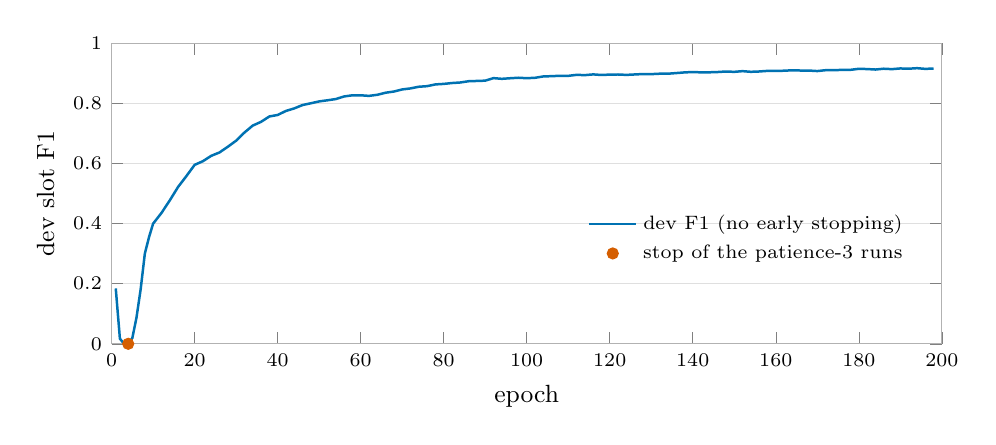
\begin{tikzpicture}
    \begin{axis}[
      width=\columnwidth, height=5.4cm,
      xlabel={epoch}, ylabel={dev slot F1},
      xmin=0, xmax=200, ymin=0, ymax=1,
      ymajorgrids, grid style={gray!25},
      axis line style={gray!60},
      tick label style={font=\scriptsize},
      label style={font=\small},
      legend style={draw=none, fill=none, font=\scriptsize, at={(0.97,0.35)}, anchor=east},
    ]
      \addplot[color=cbblue, line width=0.9pt] coordinates {
        (1,0.1841)(2,0.017)(3,0)(4,0)(5,0.0193)(6,0.0878)(7,0.1814)(8,0.2993)(9,0.3542)(10,0.3996)
        (12,0.435)(14,0.4766)(16,0.5214)(18,0.5575)(20,0.5951)(22,0.6074)(24,0.6252)(26,0.6365)
        (28,0.6554)(30,0.6756)(32,0.7026)(34,0.7258)(36,0.7382)(38,0.7561)(40,0.7611)(42,0.7745)
        (44,0.7829)(46,0.7941)(48,0.8)(50,0.8062)(52,0.8099)(54,0.814)(56,0.8226)(58,0.8265)
        (60,0.8265)(62,0.8246)(64,0.8282)(66,0.8351)(68,0.839)(70,0.846)(72,0.8494)(74,0.8549)
        (76,0.8569)(78,0.8627)(80,0.8644)(82,0.8673)(84,0.8691)(86,0.8733)(88,0.8742)(90,0.8752)
        (92,0.8836)(94,0.8813)(96,0.8832)(98,0.8849)(100,0.8834)(102,0.8847)(104,0.8893)(106,0.8901)
        (108,0.8914)(110,0.8912)(112,0.8945)(114,0.8936)(116,0.896)(118,0.8941)(120,0.8953)
        (122,0.8957)(124,0.8944)(126,0.8958)(128,0.8972)(130,0.8969)(132,0.8983)(134,0.8983)
        (136,0.9004)(138,0.9026)(140,0.9039)(142,0.9028)(144,0.903)(146,0.9039)(148,0.9056)
        (150,0.9045)(152,0.9068)(154,0.9046)(156,0.9057)(158,0.9077)(160,0.9074)(162,0.9083)
        (164,0.9097)(166,0.9089)(168,0.9088)(170,0.9071)(172,0.91)(174,0.9103)(176,0.9109)
        (178,0.9112)(180,0.9146)(182,0.9138)(184,0.9122)(186,0.9149)(188,0.9135)(190,0.9158)
        (192,0.9149)(194,0.9167)(196,0.9144)(198,0.9155)
      };
      \addplot[color=cbverm, mark=*, mark size=2, only marks] coordinates {(4,0.0)};
      \legend{dev F1 (no early stopping), stop of the patience-3 runs}
    \end{axis}
  \end{tikzpicture}
  \caption{Part 2.A diagnostic run (tiny model, lr $1\mathrm{e}{-3}$, early stopping disabled). The first epochs show a lucky peak followed by an all-O collapse where the entity-level F1 is exactly zero; the lab patience of 3 epochs stopped every run inside this phase (marker). One ATIS epoch is only 35 updates, so the patience was rescaled to 10 based on the longest stall of this curve.}
  \label{fig:diag}
\end{figure}

\begin{figure}[t]
  \centering
  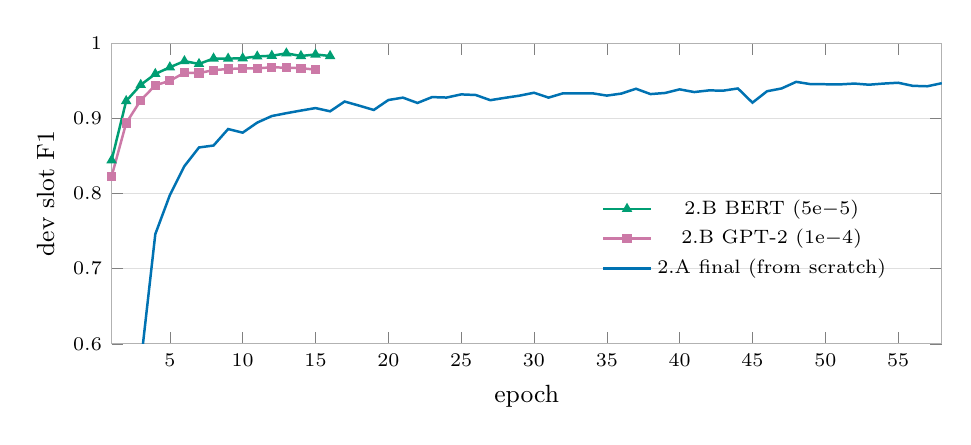
\begin{tikzpicture}
    \begin{axis}[
      width=\columnwidth, height=5.4cm,
      xlabel={epoch}, ylabel={dev slot F1},
      xmin=1, xmax=58, ymin=0.6, ymax=1,
      ymajorgrids, grid style={gray!25},
      axis line style={gray!60},
      tick label style={font=\scriptsize},
      label style={font=\small},
      legend style={draw=none, fill=none, font=\scriptsize, at={(0.95,0.35)}, anchor=east},
    ]
      \addplot[color=cbgreen, mark=triangle*, mark size=1.3, line width=0.9pt] coordinates {
        (1,0.8442)(2,0.923)(3,0.9445)(4,0.959)(5,0.9679)(6,0.9761)(7,0.9723)(8,0.9796)
        (9,0.9794)(10,0.9799)(11,0.9823)(12,0.9832)(13,0.9864)(14,0.9829)(15,0.9849)(16,0.9829)
      };
      \addplot[color=cbpurp, mark=square*, mark size=1.2, line width=0.9pt] coordinates {
        (1,0.8227)(2,0.8937)(3,0.924)(4,0.9439)(5,0.9499)(6,0.9606)(7,0.9602)(8,0.9641)
        (9,0.9656)(10,0.9664)(11,0.9664)(12,0.9679)(13,0.9673)(14,0.9667)(15,0.9647)
      };
      \addplot[color=cbblue, line width=0.9pt] coordinates {
        (1,0.0079)(2,0.296)(3,0.5735)(4,0.7459)(5,0.7978)(6,0.8364)(7,0.8612)(8,0.8638)
        (9,0.8857)(10,0.8809)(11,0.8943)(12,0.903)(13,0.9068)(14,0.9103)(15,0.9136)(16,0.9093)
        (17,0.9223)(18,0.9168)(19,0.9111)(20,0.9243)(21,0.9275)(22,0.9204)(23,0.9282)(24,0.9276)
        (25,0.9318)(26,0.931)(27,0.9241)(28,0.9272)(29,0.9301)(30,0.934)(31,0.9275)(32,0.9333)
        (33,0.9331)(34,0.9333)(35,0.9302)(36,0.9329)(37,0.9393)(38,0.9322)(39,0.9337)(40,0.9385)
        (41,0.9349)(42,0.9371)(43,0.9368)(44,0.9397)(45,0.9208)(46,0.936)(47,0.9397)(48,0.9485)
        (49,0.9454)(50,0.9453)(51,0.9451)(52,0.9462)(53,0.9447)(54,0.9462)(55,0.9473)(56,0.9432)
        (57,0.9426)(58,0.9467)
      };
      \legend{2.B BERT ($5\mathrm{e}{-5}$), 2.B GPT-2 ($1\mathrm{e}{-4}$), 2.A final (from scratch)}
    \end{axis}
  \end{tikzpicture}
  \caption{Convergence of the selected configurations (development slot F1, seed 42). The pretrained models start high and converge within 15 epochs; the from-scratch decoder needs about 50 epochs and plateaus roughly 4 F1 points below GPT-2 and 7 below BERT, which quantifies the value of pretraining on this small corpus.}
  \label{fig:conv}
\end{figure}

\bibliographystyle{../../report_template/IEEEtran}

\bibliography{nlu_refs}

\end{document}
